\chapter{Implementación}

\fancyhead[R]{7. Implementación}

\noindent\fbox{
	\parbox{\textwidth}{
    En este capítulo se definen las acciones realizadas en cada etapa del proyecto, así como los problemas que hayan podido surgir, y la experiencia una vez finalizada cada fase. 
	}
}

\section{Desarrollo en Arduino}

Para desarrollar las funciones necesarias en Arduino, se trabajará con una protoboard para realizar el prototipo y poder comprobar que todas las funcionalidades trabajan de la forma correcta. La versión de Arduino IDE en la que se realizará este proyecto es la \textbf{v2.1}, lanzada el 24 de abril de 2023. 

\subsection{Desarrollo de funciones secuenciales sin FREERTOS}

En el primer apartado del desarrollo en arduino, se programarán funciones simples para cada uno de los subsistemas, sin entrada del usuario ni de programas externos, para facilitar la comprensión de dichas funciones y agilizar la temporización de las funciones con FreeRTOS. 

\subsubsection{Sección de luces}

Para realizar el encendido y apagado de luces, lo primero es declarar los pines digitales necesarios como OUTPUT, para después variar su estado con \textbf{digitalWrite()}. El retardo, si fuese necesario, se implementará con un tiempo de 200ms entre estados mediante la función \textbf{delay}.

A continuación se muestra el circuito utilizado para comprobar que todas las funciones que se implementarán a continuación funcionan correctamente: 

\begin{figure}[H]
    \centering
    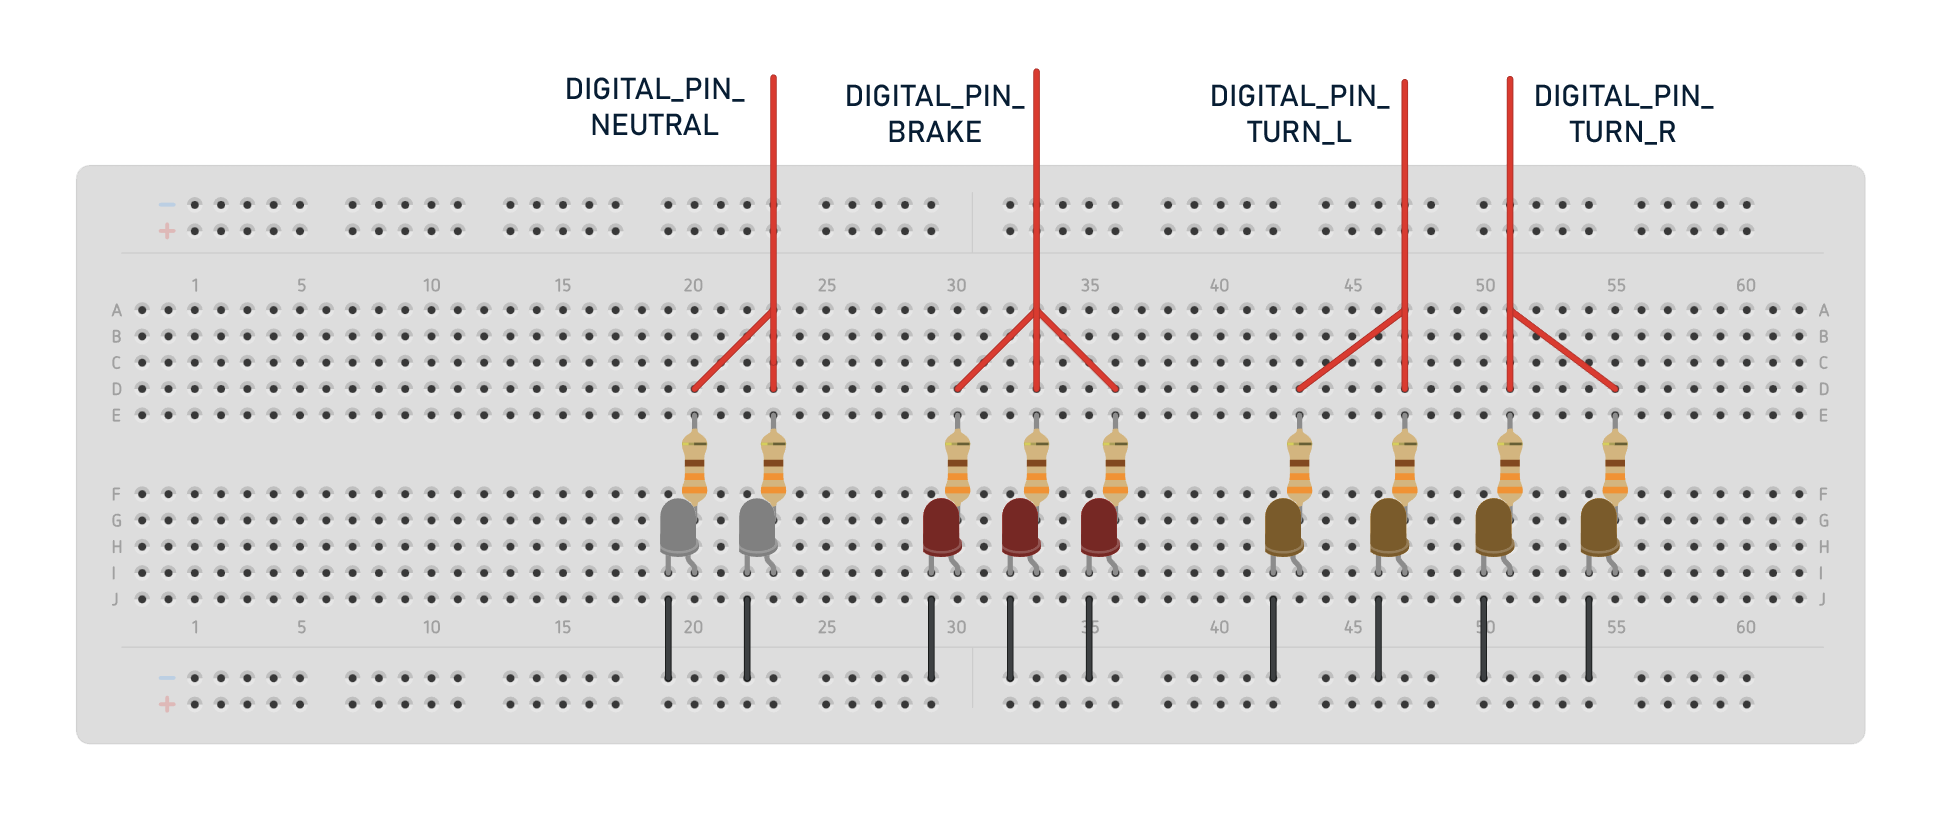
\includegraphics[width=1\textwidth]{imagenes/diagramas/luces_ard.png}
    \caption{Circuito de las luces. Elaboración propia}
\end{figure}

A partir de ahora, se distinguirá en dos tipos de funciones:

\paragraph*{Funciones de luces con parpadeo}
Estas funciones son aquellas en las que las luces varían entre encendidas y apagadas con un retardo acotado, siendo estas las necesarias para el funcionamiento y las luces de emergencia.

\begin{figure}[H]
    \centering
    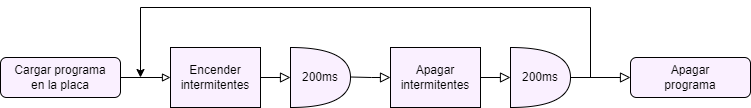
\includegraphics[width=0.9\textwidth]{imagenes/diagramas/turn_base.png}
    \caption{Diagrama de flujo de la función de luces intermitentes. Elaboración propia}
\end{figure}


\paragraph*{Funciones de luces fijas}
Las luces en estas funciones se mantienen fijas en el estado que se requiera, ya sea apagadas o encendidas, al recibir entrada del usuario (implementado directamente en la próxima sección mediante el serial). Entran en este apartado las luces de freno y las luces neutrales o cortas. 


\begin{figure}[H]
    \centering
    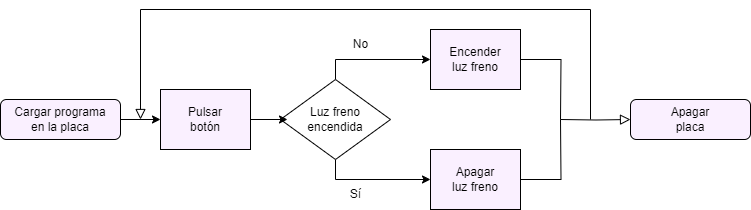
\includegraphics[width=0.9\textwidth]{imagenes/diagramas/brake_base.png}
    \caption{Diagrama de flujo de la función de luces de freno. Elaboración propia}
\end{figure}







\subsubsection{Sección de temperatura}

Para el subsistema que controla la temperatura, debemos tener en cuenta los dos termistores que se van a utilizar y cómo obtener el valor real de temperatura una vez tenemos el valor del sensor. Para ello, se debe estudiar el \textit{datasheet} del componente. A continuación se expone el circuito a utilizar:

\begin{figure}[h]
    \centering
    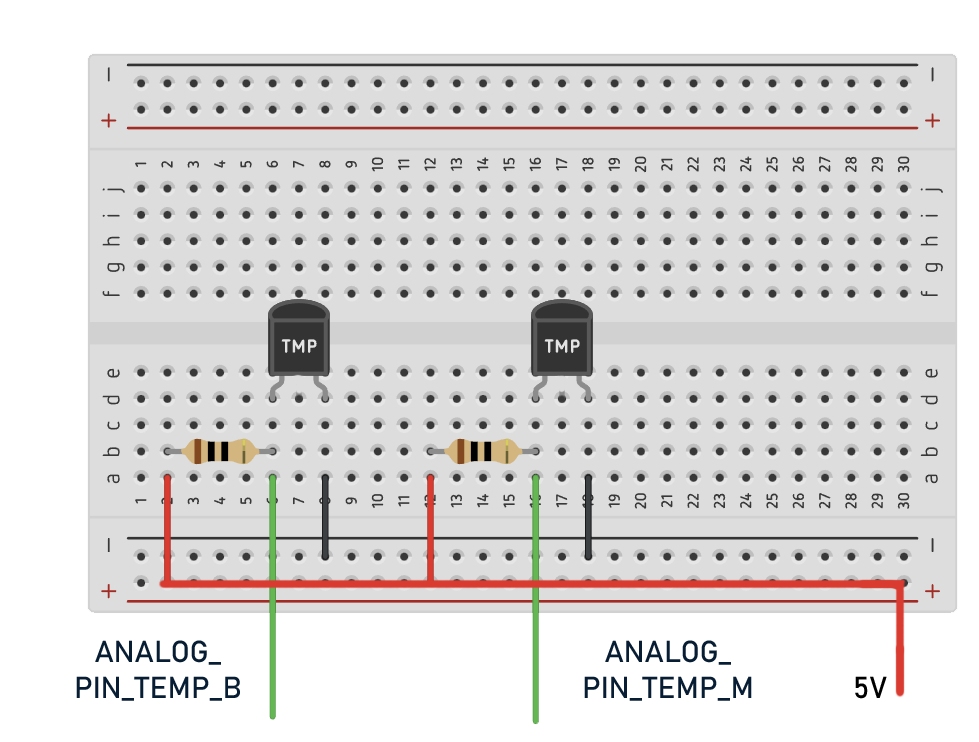
\includegraphics[width=0.7\textwidth]{imagenes/diagramas/temp_ard.png}
    \caption{Circuito de la temperatura. Elaboración propia}
\end{figure}



Para calcular la temperatura real, se deben calcular los valores necesarios mediante la ecuación de /textbf{Steinhart-Hart}, no sin antes obtener las variables \textbf{A, B } \textbf{C} requeridas para dicha ecuación \cite{termistor}.

\begin{align*}
    \frac{1}{T} = A + B\ln{R} + C(\ln{R})^{3}
\end{align*}

Donde las variables tienen los siguientes valores:
\begin{itemize}
    \item \textbf{A}: 1.11492089e-3
    \item \textbf{B}: 2.372075385e-4
    \item \textbf{C}: 6.954079529e-8
    \item \textbf{R}: R\_externa*V / V\_in-V
\end{itemize}

Una vez se tienen todos los valores necesarios, únicamente resta incluir todos estos cálculos en una función para la lectura, y crear otra función que se encargue de escribir el valor de temperatura real en el puerto serial para su visualización.

\begin{figure}[H]
    \centering
    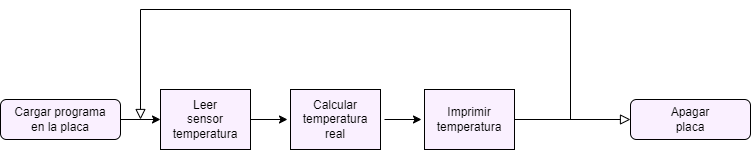
\includegraphics[width=1\textwidth]{imagenes/diagramas/temp_base.png}
    \caption{Diagrama de flujo de la función de temperatura. Elaboración propia}
\end{figure}




\subsubsection{Sección de motor}

Para el control de los motores se utilizará la placa \textbf{L928N}, como se expuso anteriormente. Esta placa simplifica el circuito y permite que no existan conexiones directas desde el Arduino Mega a los motores, pues puede provocar cortocircuitos. 

\begin{figure}[H]
    \centering
    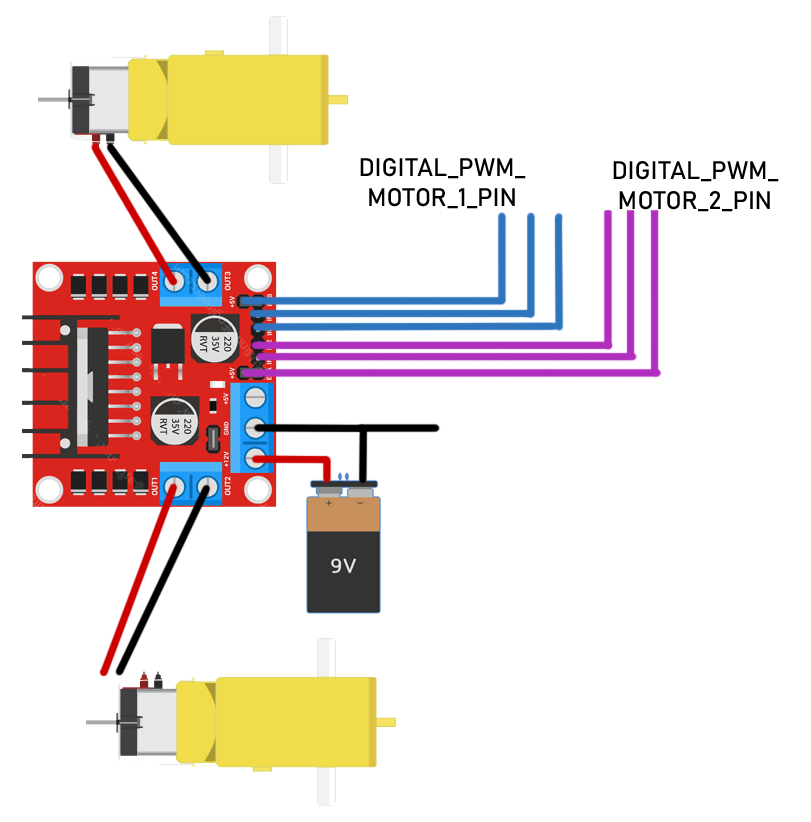
\includegraphics[width=0.6\textwidth]{imagenes/diagramas/motor_ard.png}
    \caption{Circuito de los motores. Elaboración propia}
\end{figure}

En esta función base no se utilizarán los pines de comunicaciones, por lo que mantendremos los jumper. El objetivo es únicamente comprobar que se puede encender y apagar los motores, no variar su velocidad (función que se implementará en FreeRTOS directamente, como indica el esquema inferior).

Para ello, se deben definir los pines digitales con señal PWM de ambos motores como OUTPUT, y escribir en ellos HIGH o LOW para encender o apagarlos. El control de dirección es sencillo, pues se ha realizado conectando los cables de positivo y negativo de manera inversa entre ambos motores. 

\begin{figure}[H]
    \centering
    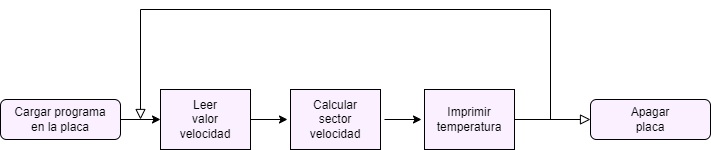
\includegraphics[width=1\textwidth]{imagenes/diagramas/motor_base.png}
    \caption{Diagrama de flujo de la función de velocidad del motor. Elaboración propia}
\end{figure}



\subsubsection{Función setup}

En esta función, que realiza la misma tarea que en Arduino secuencial, se va a declarar todas las variables globales, manejadores, colas, semáforos y tareas necesarias para el funcionamiento del programa. 

Además de estos pasos, también se deberá crear las instancias de tareas de lectura de puerto serie y temperaturas, que inician su ejecución al comenzar la ejecución del programa. 

La estructura de creación de una tarea en FreeRTOS es la siguiente. 

\begin{verbatim}
    xTaskCreate(
        NombreTarea,
        "NombreParaProgramador",
        TamanioPila,
        Argumentos,
        Prioridad,
        &manejador);
\end{verbatim}

Si bien todos los argumentos de la función \textbf{xTaskCreate} son importantes, los manejadores o \textit{handler} son decisivos para cualquier proyecto, pues permiten gestionar el estado de la función que controlan desde cualquier otro punto del código, ya sea otra función u otra tarea. 

\subsection{Desarrollo de funciones concurrentes con FREERTOS}

En este apartado se desarrollará la versión concurrente de las funciones que se programaron anteriormente, añadiendo la comunicación con el puerto serie y gestionando el uso de recursos compartidos entre los distintos procesos. 


\subsubsection{Función de manejo del serial}

Esta función será la piedra angular del programa, pues será la encargada de recibir entrada del usuario, procesar su petición y, si fuera necesario, mostrar los datos en el puerto serie (o en la interfaz gráfica en los siguientes apartados).

Se ha inicializado un semáforo que se encargue de asegurar que todas las lecturas y escrituras sobre el puerto serie estén protegidas, evitando así la pérdida de datos o pulsaciones del usuario. A continuación se detalla la sintaxis del bloqueo que impone sobre el semáforo la función del serial para facilitar la comprensión.

\begin{verbatim}
    if (xSemaphoreTake(serial_sem, (TickType_t)5) == pdTRUE) {
        value_serial = Serial.read();
        xSemaphoreGive(serial_sem);
        vTaskDelay(20 / portTICK_PERIOD_MS);
      }  
\end{verbatim}

Como se puede observar en el código, se realizan los siguientes pasos:

\begin{enumerate}
    \item La función comprueba que el semáforo no esté bloqueado en otro punto del código y, si no lo está, se adueña de él.
    \item Se realiza la lectura del serial pertinente.
    \item Se devuelve el semáforo y se añade un retardo para asegurar que no se produzca una condición de carrera. 
\end{enumerate}

Una vez se ha obtenido el valor del serial introducido por el usuario y/o la interfaz, se gestionará mediante un switch para evitar la sobrecarga del puerto serie al intentar leer de él todas las funciones. Una vez detectado el valor que corresponde a una de estas funciones, se realizarán las acciones asociadas a dicha señal, que normalmente son las siguientes:

\begin{enumerate}
    \item Comprobación del estado de la función, si el sistema a manejar está encendido o apagado.
    \item Comprobación con dependencias de otras funciones que puedan ser incompatibles con la que se llama mediante el serial.
    \item Creación o destrucción de la tarea asociada teniendo en cuenta el estado de la misma. 
    \item Limpieza de pines asociados a la tarea si fuese necesario. 
\end{enumerate}



\subsubsection{Funciones de luces}

Las funciones asociadas a la iluminación no han variado demasiado respecto a las secuenciales, aunque se han añadido restricciones entre luces de emergencia e intermitentes para que no se desincronice el parpadeo de los LEDs. También se ha acotado el retardo respecto al tiempo de acceso a los recursos mediante la variable \textbf{portTICK\_PERIOD\_MS}.

\subsubsection{Funciones de temperatura}

Las funciones y tareas referentes a las temperaturas de motor y batería han sufrido grandes cambios, entre ellos la modularización de las instrucciones.

Para realizar la lectura desde el sensor se ha creado una función que se encargue de leer el valor del sensor y calcular la temperatura real. Dicha función es llamada por la tarea de lectura de temperatura, que está ejecutándose desde que se carga el programa en la placa. 

La comunicación entre las tareas de lectura y escritura ahora se realizará mediante una cola para minimizar el uso de variables globales y agilizar el tiempo de respuesta. 

Se ha añadido también una codificación de la temperatura para distinguir entre los valores de los dos termistores a la hora de desarrollar la interfaz y distribuir los datos recibidos de manera correcta.

\subsubsection{Funcion del motor}

La función de control de velocidad del motor ha sido implementada mediante una tarea, que recibe las pulsaciones '+' y '-' para aumentar y disminuir el voltaje en doce tramos. Se ha añadido un valor inicial para designar el voltaje mínimo que requieren los motores para funcionar de manera correcta. 

El control del máximo y mínimo de velocidad se harán mediante interfaz para simplificar la comunicación, por lo que esta versión todavía no posee mecanismos de limitación de velocidad \textit{per se}, aunque al estar trabajando en un puerto analógico el máximo valor será siempre 255, por lo que existe esa restricción que evita que pueda suministrarse un exceso de voltaje al sistema. 

\begin{figure}[H]
    \centering
    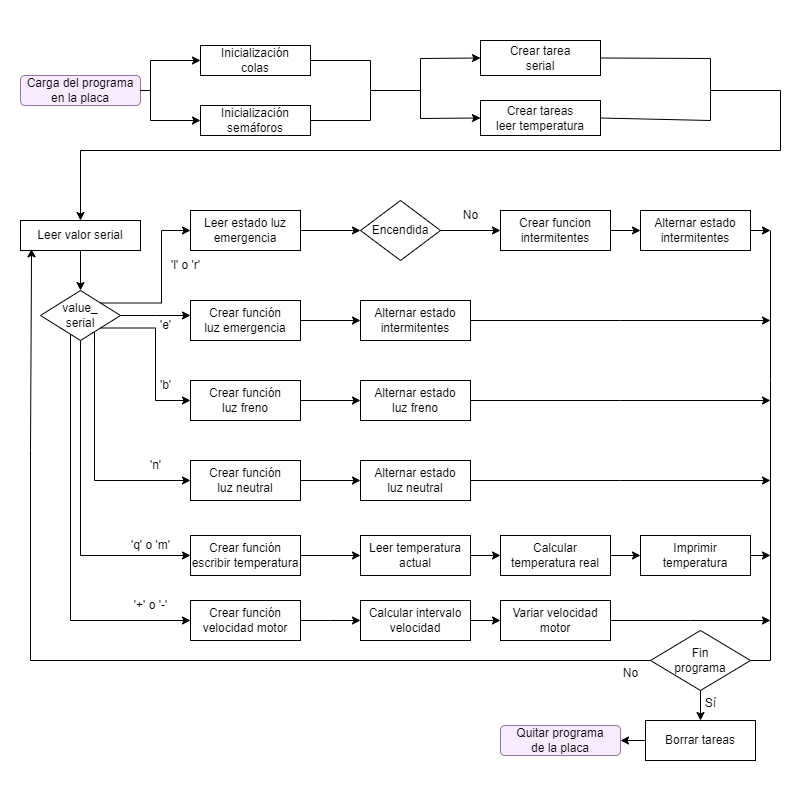
\includegraphics[width=1\textwidth]{imagenes/diagramas/Diagrama_FREERTOS.png}
    \caption{Diagrama de flujo del código con comunicación. Elaboración propia}
\end{figure}


\section{Desarrollo en Processing}

Para diseñar la interfaz en Processing se utilizará la librería ControlP5, ya mencionada anteriormente, por su facilidad de implementación de botones, ruedas y \textit{sliders}. Sería posible diseñar estas funcionalidades desde cero, ya que Processing es muy flexible, pero el uso de ControlP5 simplifica el desarrollo enormemente. 

\subsection{Desarrollo de interfaz de usuario base sin comunicaciones serie}


Antes de comenzar a programarla, lo mejor es realizar un esquema simple indicando dónde debe ir cada función y cada sección, por lo que se realiza un boceto en GIMP con dicha información:

\begin{figure}[H]
    \centering
    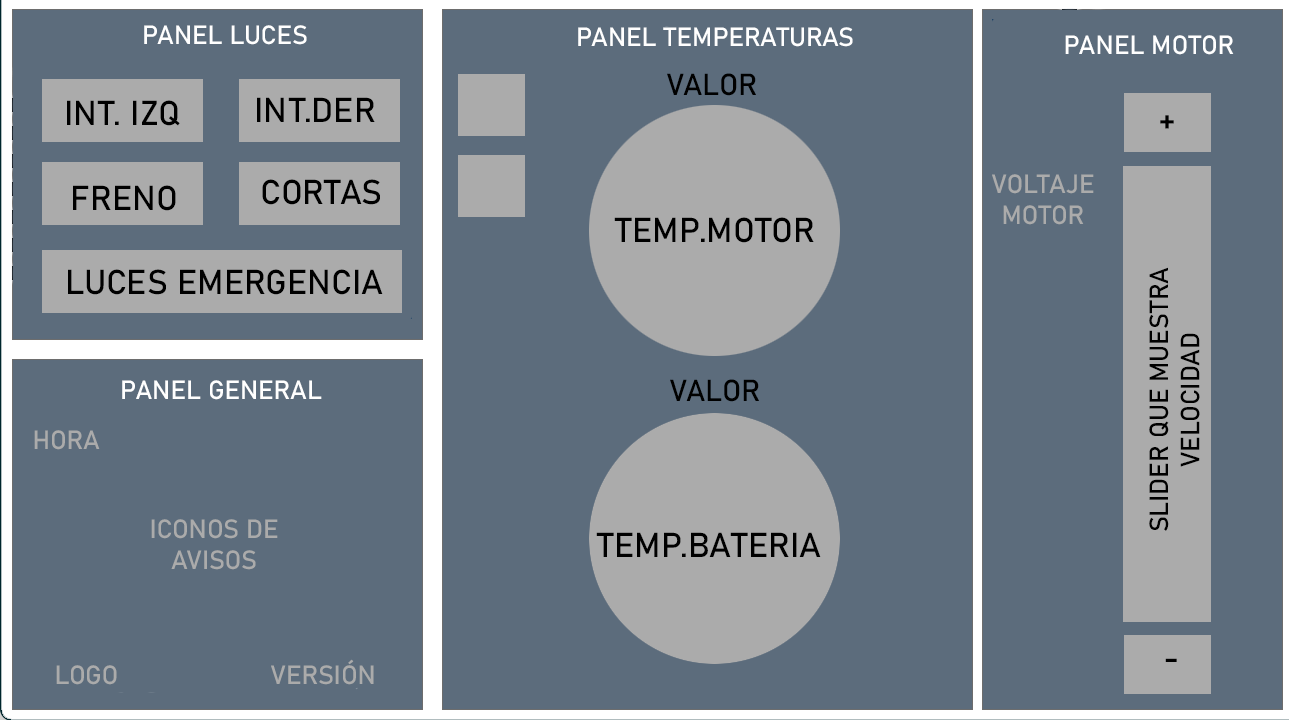
\includegraphics[width=1\textwidth]{imagenes/cargui_base.png}
    \caption{Boceto de la interfaz gráfica. Elaboración propia}
\end{figure}

Una vez se tiene una idea general de lo que se va a realizar, es el momento de programar y diseñar el boceto. Se segmentará el desarrollo en secciones para menor granularidad de tareas.

\subsubsection{Panel de luces}

El panel de luces es sencillo, pues únicamente constará de cinco botones. La programación de dichos botones se realizará mediante la función \textbf{addButton}. A continuación se expone el código para la declaración de uno de estos botones:

\begin{verbatim}
    cp5.addButton("IntermitenteIZQ")
    .setSize(180,80)
    .setPosition(20, 60)
    .setFont(font)
    .setLabel("Intermitente \n    izquierdo")
\end{verbatim}

Si bien todas las propiedades son importantes, el nombre que se le da al botón, en este caso "intermitenteIZQ", es extremadamente importante, pues será el nombre de la función que se llamará cuando se pulse el botón, y permita asociarle una acción. Dicha función se implementará durante la próxima sección.

\subsubsection{Panel general}

El objetivo de este panel será proveer de información al usuario con un solo vistazo mediante iconos que se iluminarán dependiendo de las circunstancias, véase un intermitente encendido, exceso de temperatura, etcétera. También incluirá datos relevantes de la versión de la interfaz como su autoría y la versión en la que se encuentra. 

Durante el desarrollo de este panel, surgió un problema a la hora de visualizar los iconos encendidos y apagados, pues no se podía eliminar una imagen y mostrar la del estado en el que se encontraba el sistema. Para solucionar esto se añadió una jerarquía de imágenes, mostrando por defecto el icono de apagado, y superponiendo el icono de encendido cuando fuera necesario.

\subsubsection{Panel de temperatura}

Este panel es posiblemente el más complejo de implementar. Si bien existen otras herramientas y librerías para la visualización de valores de temperatura, se va a adaptar una función de ControlP5 para mantener el estilo coherente con el resto de funcionalidades. 

Se trabajó con el objeto \textbf{knob}, que normalmente se utiliza para seleccionar un valor en un rango mediante el deslizamiento del ratón. Dicho valor, que normalmente es variable por entrada del usuario, se tomará de los datos que envíe la placa por el puerto serie en próximas versiones, además de eliminar la posibilidad de introducir el valor de manera manual. 

En este momento surgieron varios problemas con el tratamiento de temperaturas, pues ambos visores mostraban valores iguales. Esto supuso un cambio en la función de temperatura, pues el problema era que no existía diferenciación entre los valores que mandaban ambos termistores a la GUI. Para poder subsanar este error se introdujo un caracter al final del valor de temperatura de cada uno de los termistores, pudiendo así identificar a cuál de ellos correspondía el valor recibido. También se añadió un método para poder eliminar ese caracter distintivo y recuperar el tipo flotante de la temperatura, y así poder mostrarlo en el visor. 

Una vez implementados los dos visores de temperatura, se añadieron botones para encender y apagar la escritura de temperaturas, además de añadir la visualización numérica de los valores.

\subsubsection{Panel de motor}

Para realizar la sección de control de velocidad de motor se implementará un visor desde cero, realizado mediante un array de figuras (en este caso rectángulos) que se iluminarán dependiendo del valor de velocidad que tenga el sistema en el momento. Se podrá aumentar o disminuir la velocidad pulsando los botones '+' o '-', así como encender y apagar el motor de la misma manera. 

El voltaje del motor se mostrará de manera aproximada debido a la imposibilidad de incluir un sensor de voltaje en el sistema, basándose en el mínimo y máximo voltaje con el que trabajan los motores que se utilizan, y el voltaje que aporta la batería. 

\begin{figure}[H]
    \centering
    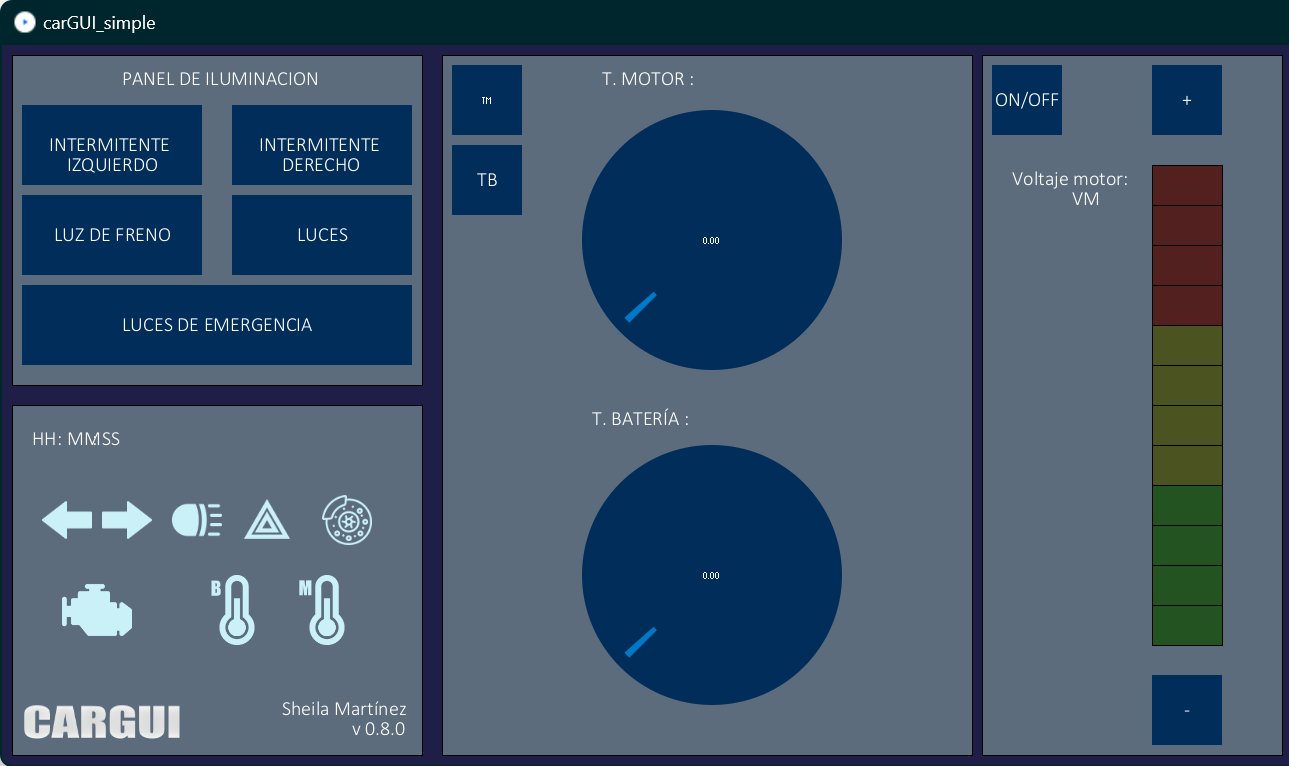
\includegraphics[width=1\textwidth]{imagenes/cargui_simple.png}
    \caption{Esqueleto de la interfaz sin funcionalidad. Elaboración propia}
\end{figure}



\subsection{Desarrollo interfaz de usuario con comunicaciones serie}

El último paso de la implementación del código se hará trabajando mayormente en la interfaz. Se añadirá lectura del puerto serie, se mejorarán los grafismos y se incluirán las funciones que no se han podido añadir antes, dotando de funcionalidad a todo el sistema. 

\subsubsection{Comunicación con el puerto serie}

El primer paso para comunicar Arduino y Processing es la conexión de este último al puerto serie, utilizando la librería \textbf{processing.serial}. Para poder enviar los avisos de pulsaciones de botones se trabajará con las funciones asociadas a estos, enviando el valor correspondiente al botón hacia la placa, donde será procesado.

Por otro lado, los datos recibidos de la placa serán procesados y mostrados en sus respectivos lugares gracias a la codificación que se le ha incluido, por ejemplo, a las temperaturas. 

\subsubsection{Mejora visual de la interfaz}

Para evitar que la interfaz quede demasiado escueta se han diseñado imágenes de cada uno de los botones, así como iconos para mostrar el estado de los sistemas en el panel general. También se incluye un grafismo de un vehículo en el que se mostrarán las distintas luces encendidas en tiempo real, emulando lo que se vería en una maqueta real. 

Además, los visores de temperatura ahora muestran mediante un degradado el rango de temperatura en el que se encuentran.

A continuación se muestra una imagen del programa con plena funcionalidad:

\begin{figure}[H]
    \centering
    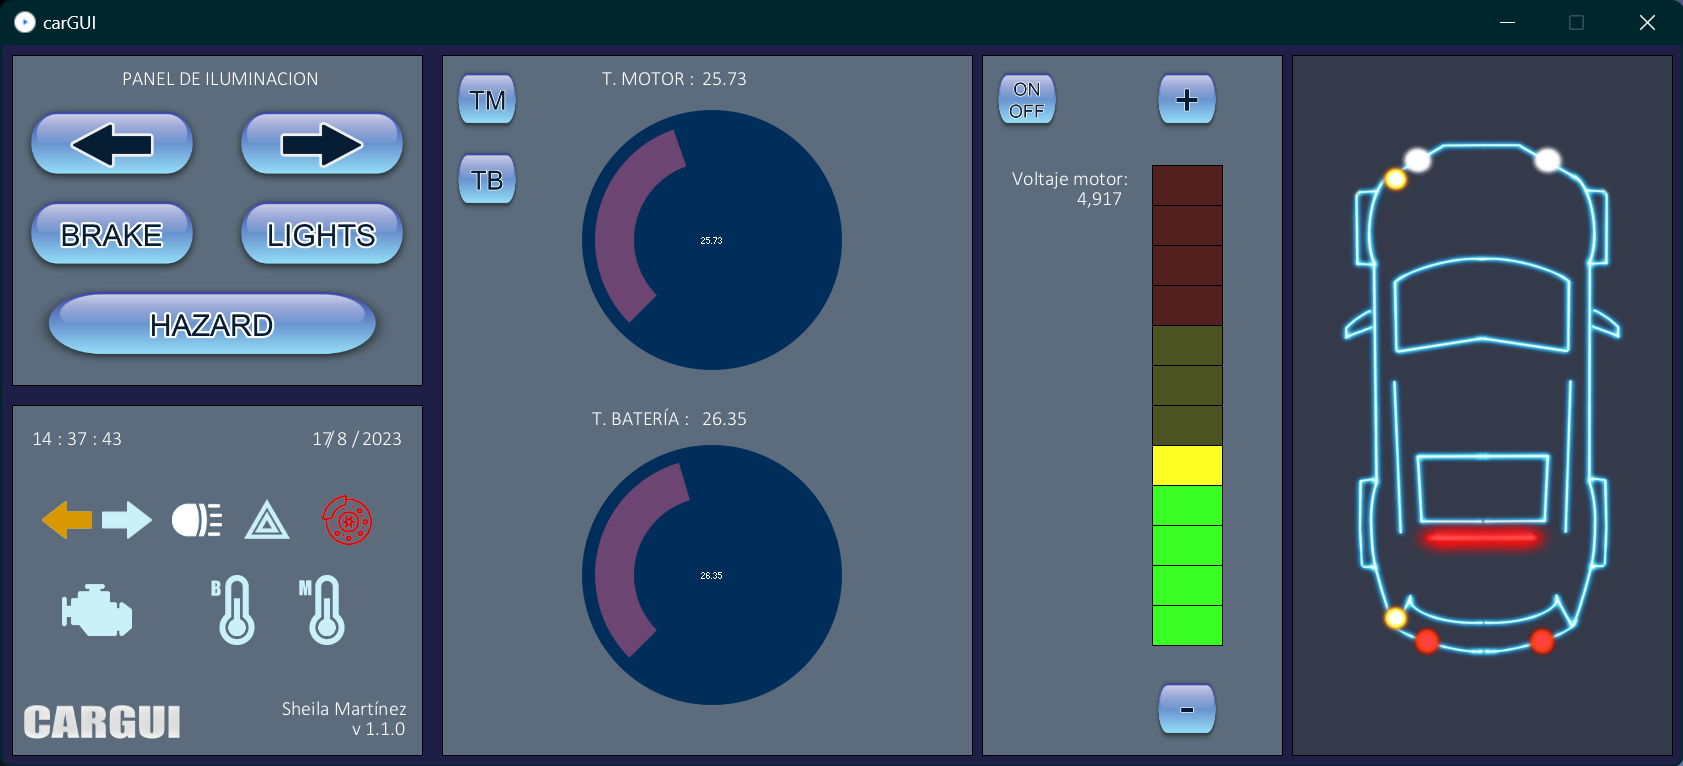
\includegraphics[width=1\textwidth]{imagenes/cargui_final.png}
    \caption{Interfaz finalizada con conexión a arduino. Elaboración propia}
\end{figure}


\section{Depuración, limpieza y documentación del código fuente}

Una vez realizado todo el código para la interfaz y la placa, se debe realizar una depuración del mismo. Para comprobar el funcionamiento correcto de la aplicación se han realizado pruebas de carga, iniciando todas las funciones en la intefaz y comprobando que no existan fallos en la concurrencia. Al realizar dichas pruebas han aparecido problemas con las temperaturas y las luces que, al ejecutarse simultáneamente, provocaban que la temperatura variase de uno a dos grados al encenderse, por ejemplo, los intermitentes. Dicho problema existía por el hecho de estar conectadas a la misma tierra, lo cual generaba una diferencia de potencial que cambiaba el valor de la temperatura. Este error se ha visto subsanado al añadir otra tierra diferente para ambos termistores, independientemente de las luces. 

También han surgido problemas por la relación entre las funciones de intemitentes y luces de emergencia al trabajar ambas sobre los mismos pines. El problema se presentaba cuando las luces de emegencia estaban encendidas y se activaba uno de los dos intermitentes, pues se desincronizaban las luces de ambas direcciones. La manera de arreglar este problema ha sido añadir un control en la función de serial indicando el estado de las luces de emergencia y, si estas están activas, no crear la función de los intemitentes. 

Tras solucionar los errores y realizar la depuración del código, se ha organizado en secciones para simplifican la lectura del mismo, así como uniformar el formato de las funciónes y los nombres de las variables. También se ha añadido un archivo de cabeceras para todas las variables y declaración de funciones, semáforos, colas y tareas, además de documentar dicho archivo para indicar las variables que reciben y retornan las funciones y tareas, así como una breve descripción de su funcionamiento y/o utilidad. 


\section{Montaje en maqueta} 

En este apartado se detallarán los pasos seguidos para integrar todos los componentes en una maqueta, así como todos los problemas y errores que se han cometido durante el montaje. La comunicación con la maqueta se realizará por cable, captando las órdenes desde el ordenador mediante los botones de la interfaz, y siendo esta quien enviará la orden al programa por el puerto serie, configurado a 9600 baudios, para ser recibida por medio de un USB por la placa, que ejecutará las acciones pertinentes.\newline

 Se ha comenzado con el prototipo que se ha utilizado para desarrollar el código de la aplicación, que figura en la siguiente imagen.

\begin{figure}[H]
    \centering
    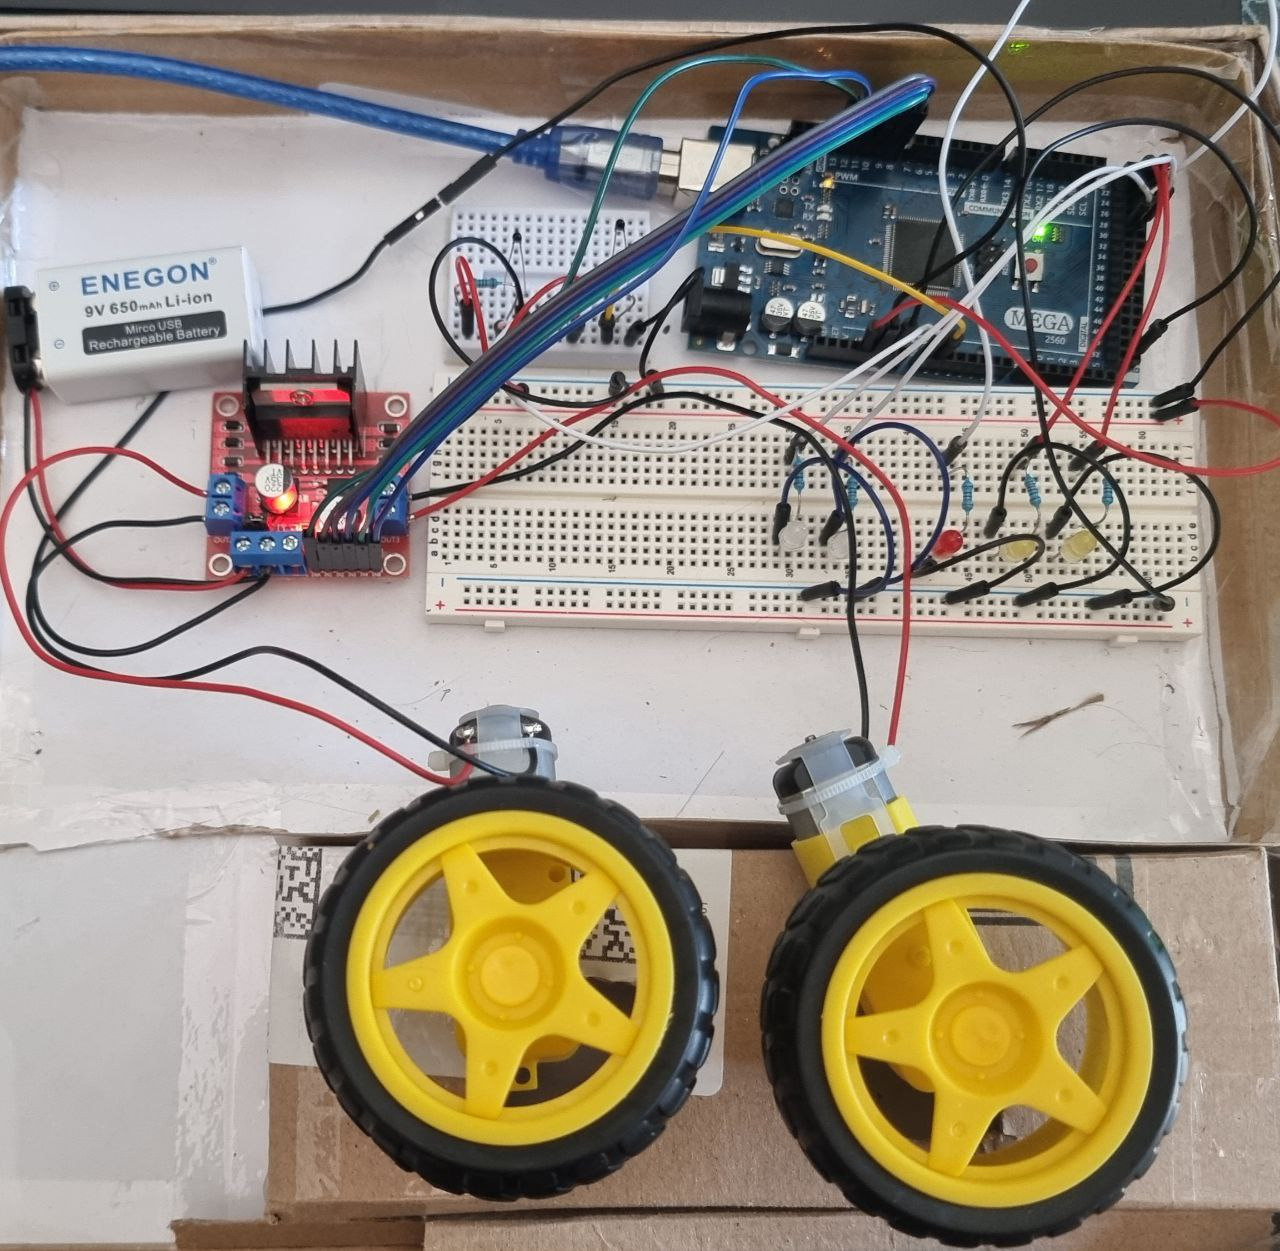
\includegraphics[width=1\textwidth]{imagenes/montaje/prototipo.jpg}
    \caption{Prototipo para el desarrollo de funciones. Elaboración propia}
\end{figure}

 Tras extraer todos los componentes de dicho prototipo, se ha realizado la soldadura de componentes para las luces y los termistores, añadiendo un recubrimiento termoretráctil para cubrir los puntos de soldadura y cables que quedasen al aire. Esta fase se ha alargado más de lo necesario debido a problemas con los componentes, pruebas con el soldador y fallos de cálculo en cantidades de materiales necesarios, pero finalmente se ha conseguido un resultado aceptable. 

 \begin{figure}[H]
    \centering
    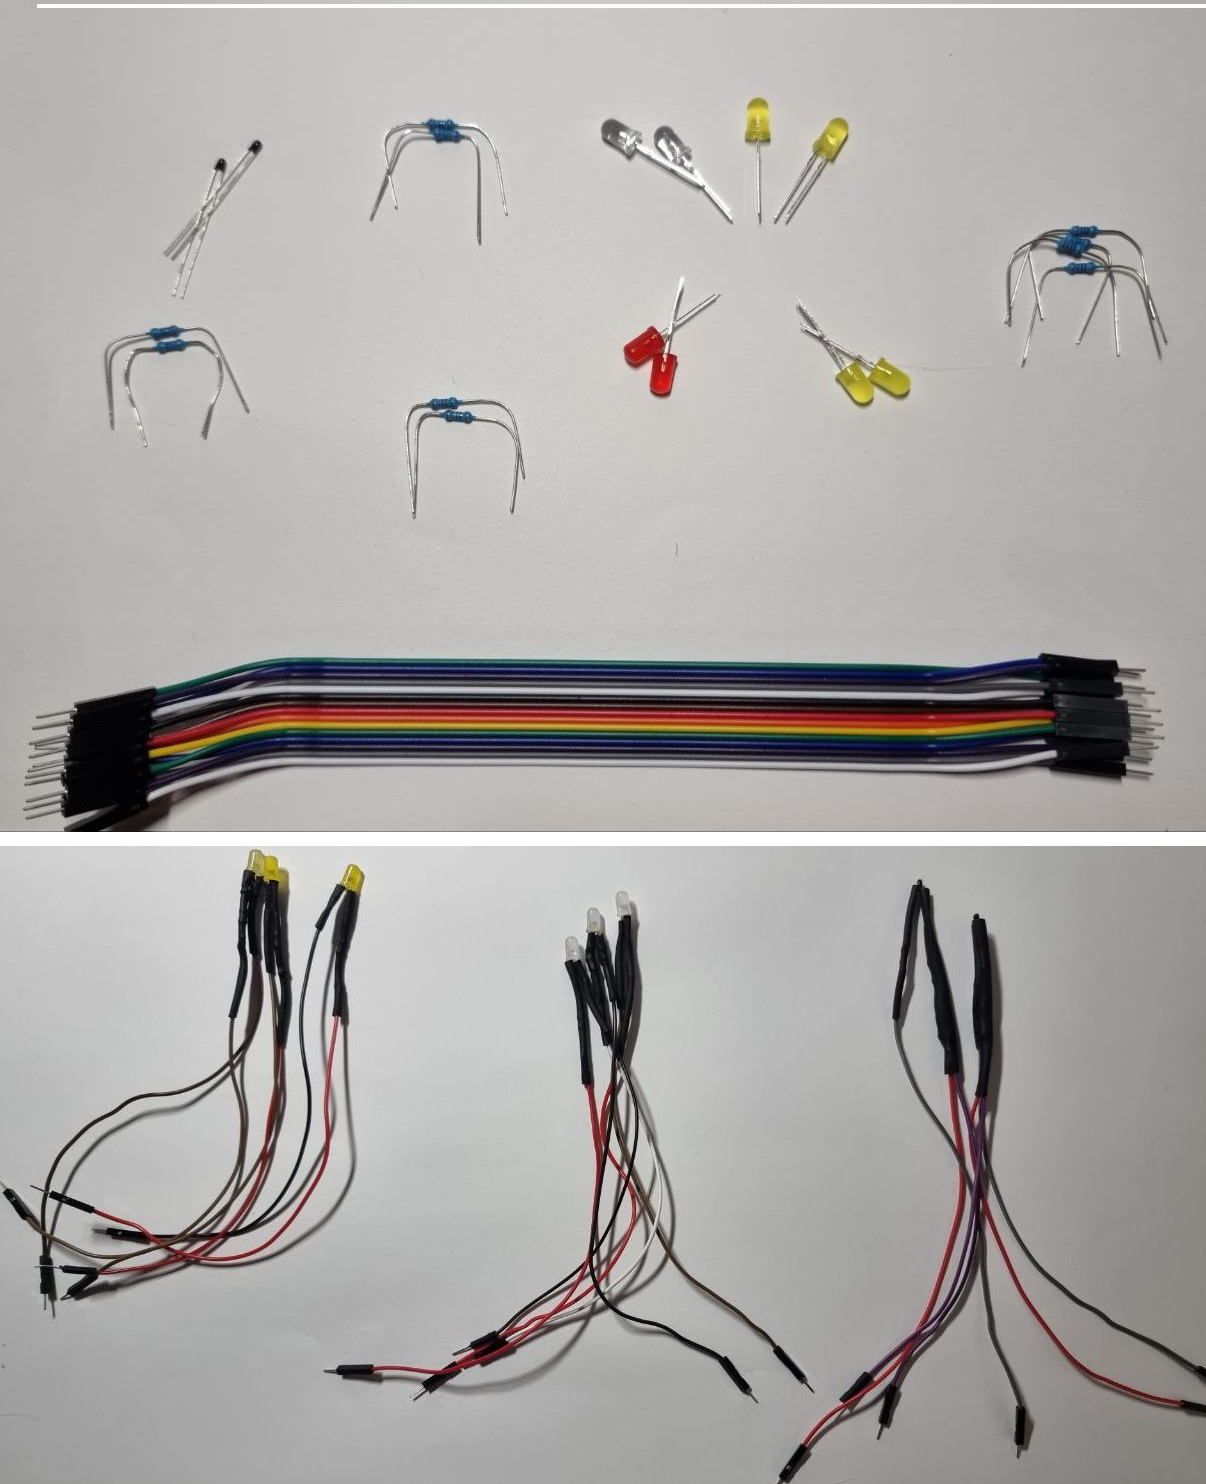
\includegraphics[width=1\textwidth]{imagenes/montaje/luces.jpg}
    \caption{Construcción de los circuitos de iluminación y temperatura. Elaboración propia}
\end{figure}



Una vez realizadas las soldaduras, se ha intentado acomodar todo dentro del coche que se escogió durante la planificación, de escala 1/24, pero aunque las mediciones realizadas parecían demostrar que era suficiente espacio, no se tuvo en cuenta la cantidad de cables del circuito. Por tanto, y viendo que no había posibilidad de implementar el circuito dentro de la maqueta, se buscó un coche escala 1/18, con el consiguiente tiempo de espera y retraso en la producción. 

Cuando llegó el siguiente modelo se desmontó entero, dejando únicamente la carrocería, la base de la maqueta y las ruedas. Una vez vacío el coche, se ubicó y reforzó el cableado mediante silicona caliente, fijándolo a la carrocería. Se añadieron también los termistores ubicados cerca de su lugar final, así como también se añadieron los dos motores que se indicaron en la planificación. 

Tras realizar las pruebas para comprobar que todos los sistemas funcionasen, surgieron problemas con los dos motores, pues los ejes no estaban adaptados a las ruedas que se iban a utilizar (las de la maqueta), eran demasiado grandes para el modelo, y además requerían de demasiada potencia para comenzar a funcionar debido a su baja eficiencia. Vistos estos problemas, se realizó la compra de unos motores más pequeños y eficientes, normalmente utilizados para modelismo y vehículos radiocontrol de media-alta gama. Estos motores mostraron buen rendimiento y un valor de voltaje muy inferior al requerido por los anteriores dejando mucho más espacio disponible en la parte frontal del vehículo, por lo que se implementaron en el circuito. 



Ya con todos los componentes instalados en la maqueta, se procedió a intentar integrar el arduino para un aspecto más limpio, añadiendo una caja de plástico debajo de la maqueta para facilitar la manipulación de los pines y permitir que la alimentación llegase a la placa, cosa que, de haber estado esta dentro de la maqueta, hubiera sido imposible. 

\begin{figure}[H]
    \centering
    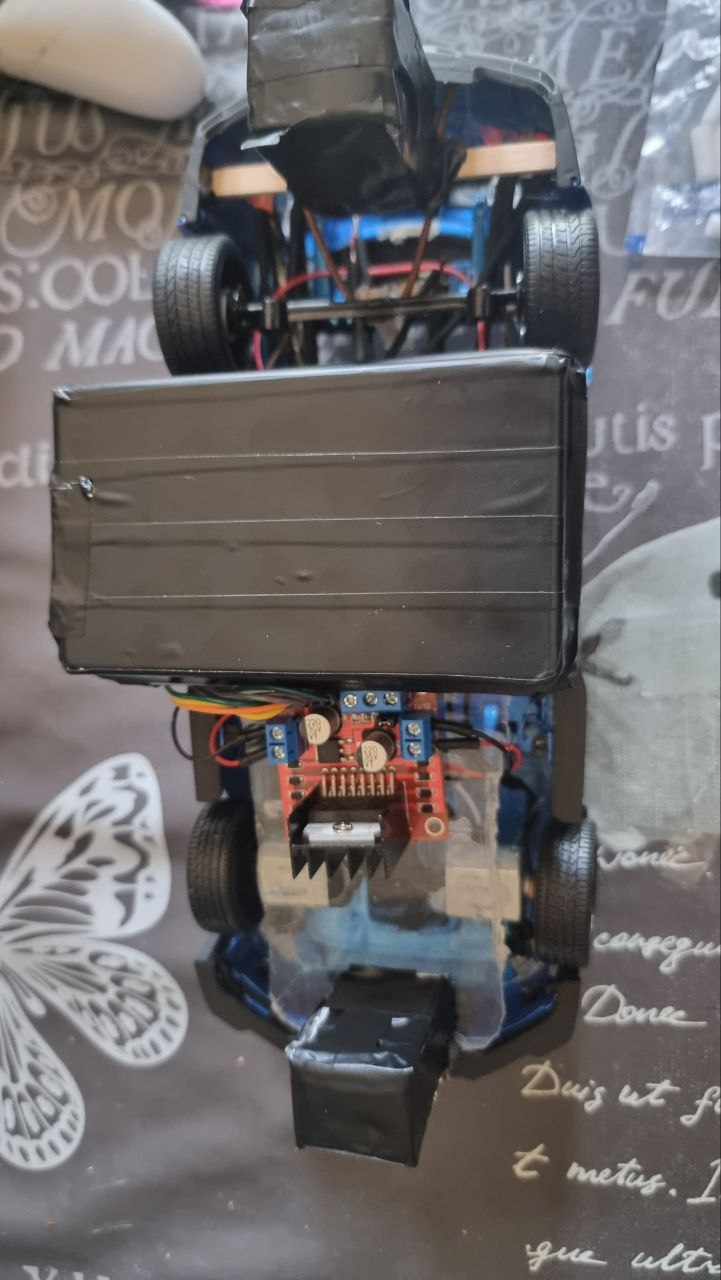
\includegraphics[width=0.6\textwidth]{imagenes/montaje/ensamblado.jpg}
    \caption{Parte inferior de la maqueta, ya con la caja de plástico integrada. Elaboración propia}
\end{figure}

El último paso fue añadir unos soportes para que las ruedas no tocasen el suelo, e intentar dejar los pesos de la zona delantera y trasera lo más equilibrados posibles. 
\begin{figure}[H]
    \centering
    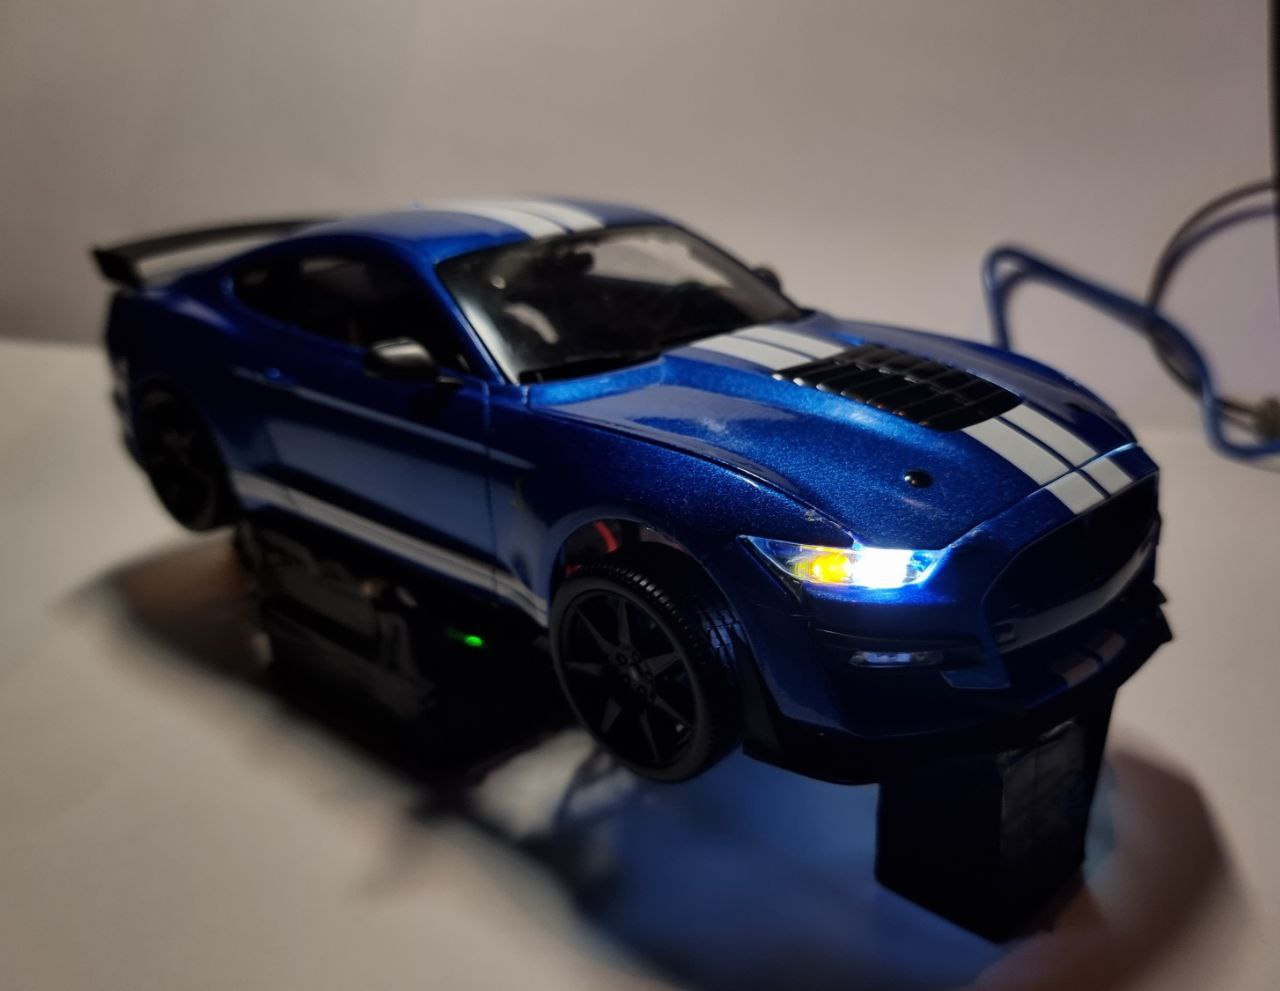
\includegraphics[width=1\textwidth]{imagenes/montaje/maqueta_final.jpg}
    \caption{Aspecto final de la maqueta mientras están activas las luces cortas e intermitente. Elaboración propia}
\end{figure}



Terminada esta tarea, queda completa la implementación del proyecto, aunque hay algunas funciones que no han podido implementarse que se detallarán a continuación.

\subsection*{Medidor de voltaje en tiempo real}

Si bien esta función parecía sencilla en un principio, el hecho de usar baterías para medir el voltaje que se le proporciona a los motores generaba un problema de compatibilidad con el módulo de medición de voltaje y la placa L928N. Un medidor de voltaje hubiera incluido demasiado trabajo y una inversión en diferentes componentes que aumentaban el coste del proyecto y sobrepasaban el presupuesto que se había pensado en un principio, que ya se había superado al tener que comprar un coche de mayor tamaño. 

Este problema produjo una cascada de funciones que no pudieron desarrollarse, la mayoría relacionadas con la batería.

\subsection*{Carga, autonomía y voltaje de la batería}

Las funciones relacionadas con el estado de las baterías requerían de un medidor de voltaje y otro de corriente, pues no existe manera aproximada de calcular el voltaje que se provee a los motores, necesario para obtener el porcentaje de batería restante ni la autonomía. Se ha intentado realizar otros métodos para implementar estas funciones sin éxito, por lo que, debido al tiempo restante en la planificación, se ha preferido eliminar estas funciones del proyecto. 

\subsection*{Tracción total}

Aunque en un principio se quiso implementar la tracción en ambos ejes, al realizar el montaje e incluir los componentes se han encontrado problemas a la hora de utilizar los motores que se indicaron en la planificación y, al cambiar a los otros motores, no se ha podido implementar por no tener doble eje, por lo que se ha preferido implementar únicamente tracción delantera. 